\section{Background}
\label{sec:background}

\HA{moved, will put in perfect place after finishing design}
Modern container registries such as Google Container Registry~\cite{GoogleContainerRegistry} use cloud storage as their backend Docker image storage systems. 
Users push and pull Docker images to and from their repositories stored on cloud storage. 
To facilitate a fast and high-availability service, container registries use regional private repositories across the world.  
This geographical distribution allows users to store images close to their compute instances and experience a fast response time. 
For example, IBM's Container Registry setup spans five regions~\cite{dockerworkload}. 

\HA{moved, will put in perfect place after finishing design}
On-cloud global deduplication software is widely adopted by cloud enterprises for reducing cloud storage consumption and overall storage cost. 
For example, StorReduce~\cite{storreduce_purestorage}, the deduplication software choice of Google cloud and AWS, 
performs in-line data deduplication transparently and resides between the client's application and the hosting cloud storage.

\HA{moved, will put in perfect place after finishing design}
Intuitively, such deduplication techniques can be applied to eliminate redundant data from the Docker image storage system.  
Except, the Docker image dataset is different from the common data stream. 
They are compressed archival files.
To eliminate file-level redundancy from the compressed layer files, changes must be made to these deduplication methods. 
Such changes should recognize the compression formats, perform decompression before feeding the data to a block-level or file-level deduplication process. 
Otherwise, the deduplication ratio would be very low since compressed files have a very low deduplication ratio. 

\subsection{Docker, Docker registry, and Registry backend storage systems}
Docker~\cite{docker} is a popular virtualization technology that extends traditional OS containers with higher level functionalities.
It allows to efficiently package an application and its runtime dependencies in a container image to simplify and automate application deployment~\cite{slacker}.



\begin{figure}
	\centering
	% Requires \usepackage{graphicx}
	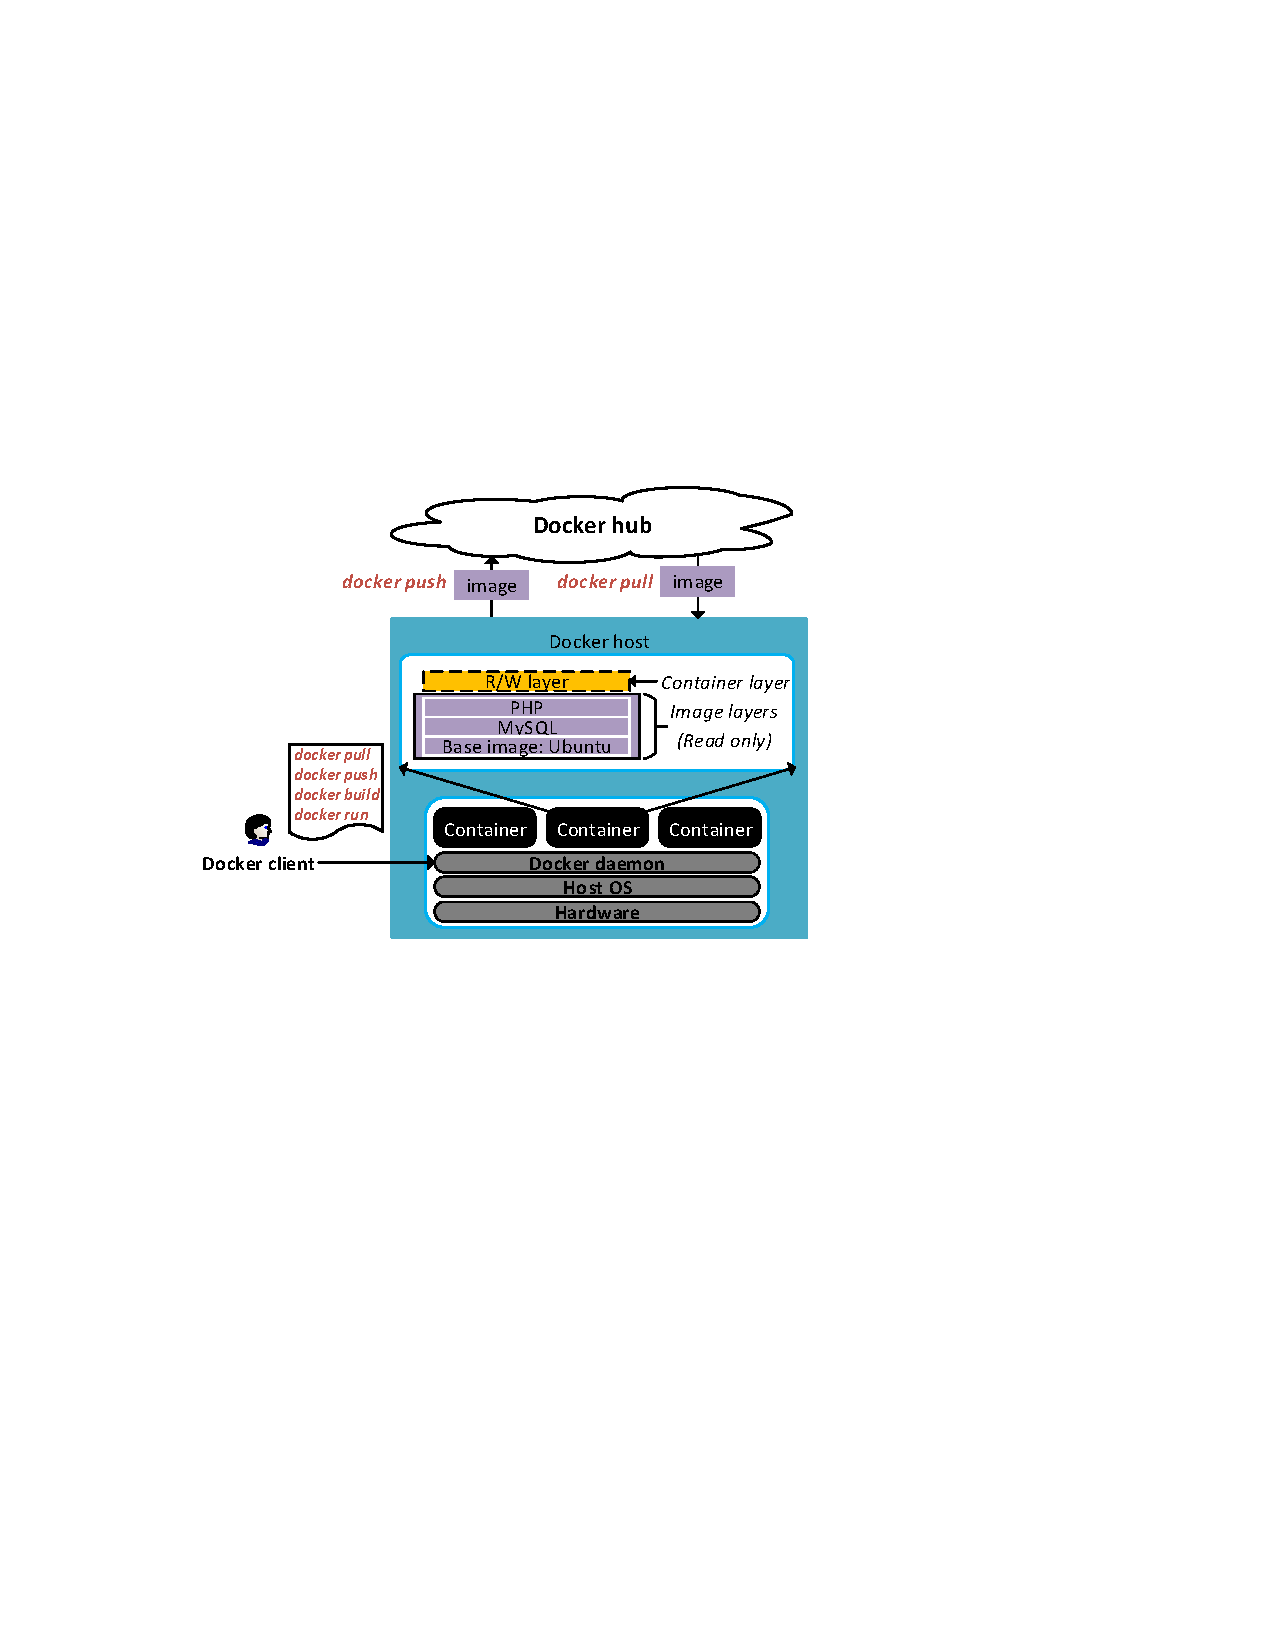
\includegraphics[width=0.5\textwidth]{graphs/fig-docker-architecture}
	\caption{Docker ecosystem
%	\lrcomment{We need to update the figure to capture
%	all the main interactions between the components and remove some unneeded
%	detail, \eg official and unofficial repositories\nancomment{addressed}}
	}
	\label{fig-docker-architecture}
\end{figure}

As shown in Figure~\ref{fig-docker-architecture}, a typical Docker setup consists of three main components: \emph{client}, \emph{host}, and \emph{registry}.
Users interact with Docker using the Docker client which, in turn, sends commands to the Docker host.
The client can be co-located on the host machine. 
The Docker host runs a daemon process that implements the core logic of Docker and is responsible for \emph{running} containers from locally available images.
If a user tries to launch a container from an image that is not available locally, the daemon \emph{pull}s the required image from the Docker registry.
Additionally, the daemon supports \emph{building} new images and \emph{pushing} them to the registry.

The Docker registry is a platform for storing and distributing container images.
It stores images in \emph{repositories}, each containing different versions (\emph{tags}) of the same image, identified as \texttt{<repo-name:tag>}.
For each image, the Docker registry stores a \emph{manifest} that describes, among other things, which layers constitute the image.
The manifest is a JSON file, which contains the runtime configuration for a container image (\eg target platform and environment variables) 
and the list of layers which make up the image.
Layers are identified via a digest that is computed as a hash (SHA-256) over the uncompressed content of the layer and stored as compressed archival files.
Image layers are stored as compressed archival files and image manifests as JSON files.

Docker Hub is one of the most popular public registries, supporting both public and private repositories, via which users can upload, search, and
download images~\cite{docker-hub}.
In Docker Hub, the user repositories are namespaced by user name, i.e., ``$\langle username\rangle/\langle repository name \rangle$", while the
official repositories, which are directly provided by Docker Inc. and partners are called ``$\langle repository name \rangle$".

Modern Docker registry identifies and addresses a layer with a digest that is computed based on the uncompressed layer's content (e.g., SHA-256).
Identifying layers by their content allows the registry to store only one instance of a layer even if it is referenced by multiple images. 
However, if at least one file differs in two otherwise identical layers, the two layers are treated as different and stored separately.

%\paragraph{Images and layers}
At the center of Docker is the concept of container images for packaging, distributing, and running applications.
A Docker image consists of an ordered series of \emph{layers}.
Each Docker layer contains a subset of the files in the image and often represents a specific component/dependency of the image, \eg a shared library.
Layers can be shared between two or more images if the images depend on the same layer.
Image layers are read-only.
When users start a container, Docker creates a new \emph{writable layer} on top of the underlying read-only layers (Figure~\ref{fig-docker-architecture}).
Any changes made to files in the image will be reflected inside the writable layer via a copy-on-write mechanism.


\subsection{Cloud Storage and Deduplication}
 
Most existing cloud storage providers employ data deduplication techniques to eliminate redundant data, same data stored more than once. 
Deduplication techniques significantly reduce storage needs and therefore reduce storage costs and improve storage efficiency. 
Data deduplication works by storing duplicate data chunks only once, keeping only the unique data chunks. 

Current cloud providers deploy a cross-user client-side fixed-size-chunk-level data deduplication that delivers the highest deduplication gain~\cite{pooranian2018rare}. 
These approaches maximize the benefit of deduplication: 
The cross-user data deduplication treats cloud storage as a pool shared by all the cloud users, because the potential for 
data deduplication is the highest as the probability for redundancies and duplicates is higher the more inclusive the shared pool. 
The client-side data deduplication is to ensure that only unique files are uploaded, to save network bandwidth, by having the client send a duplicate check request. 
The fixed-size-chunk-level specifies that a fixed-size chunk is the unit for checking for duplicates on cloud storage.

Google cloud and AWS employ StorReduce, a deduplication software that performs in-line data deduplication transparently and resides between the client's application and the hosting cloud storage. StorReduce provide 80-97\% storage and bandwidth reduction to the cloud providers~\cite{StorReduce_google}.


server-side data deduplication?

\subsection{Web/Proxy cache}
Caching is a technique widely leveraged to reduce bandwidth and load off of highly loaded bottleneck backends by temporarily storing frequently requested data. 
Caching can be introduced at the client, in between clients and servers as a proxy, or at the server side. 
Proxy caches are efficient in reducing traffic from bottleneck backends by cooperatively serving previously requested and saved data without it going all they way to the backend. 
The client therefore, experiences improved response times.

The Docker client inherently caches layers at the client. This way, the Docker daemon only pulls layers that are not available on the host machine. 

Examples of open-source web (HTTP) proxy caches include Nginx~\cite{?}, Squid~\cite{?}, and Varnish~\cite{?}. Other software used for caching include Memcached~\cite{?}, an open-source distributed in-memory key-value store that works as a caching system and Redis~\cite{?} which is an open-source key-value store that works as an in-memory store and as a cache.



\subsection{Apply traditional deduplication approaches to registries?}



\subsection{Use-cases of Slimmer}

\paragraph{Production registries} Google, IBM,

\paragraph{Private registries}

\paragraph{Enable deduplication technique handle versatile data streams without performance degradation}

